\documentclass[aspectratio=169,11pt]{beamer}
% Build:  tectonic slides.tex     (figures and colours are shared with ../final_report)
\usepackage{booktabs}
\usepackage{pgfplots}
\pgfplotsset{compat=1.18}
\newcommand{\figW}{6.8cm}      % one panel of a two-panel figure
\newcommand{\figH}{5.0cm}
\newcommand{\figLegendFont}{\tiny}
\newcommand{\figSep}{1.3cm}
\newcommand{\figWone}{6.4cm}
% One colour scheme and one set of plot styles for the report and the slides.
% Colours: Okabe-Ito (colour-blind safe). Every series also has its own mark, line style or position label, so the
% figures stay readable when printed in greyscale.
\definecolor{cFT}{HTML}{000000}      % full fine-tuning: black
\definecolor{cAttn}{HTML}{0072B2}    % attention LoRA: blue
\definecolor{cMLP}{HTML}{E69F00}     % MLP LoRA: orange
\definecolor{cBoth}{HTML}{009E73}    % attention + MLP LoRA: green
\definecolor{cAccent}{HTML}{D55E00}  % highlights: vermilion
\definecolor{cGrey}{HTML}{7F7F7F}
\usepgfplotslibrary{groupplots}
\usetikzlibrary{arrows.meta,positioning,calc}
\pgfplotsset{repaxis/.style={
  tick label style={font=\footnotesize}, label style={font=\small}, title style={font=\small\bfseries, yshift=-3pt},
  x tick label style={font=\footnotesize}, grid style={cGrey!30}, axis line style={cGrey}, tick style={cGrey},
  every axis plot/.append style={line join=round}}}
\providecommand{\figW}{0.49\textwidth}   % width of one panel of a two-panel figure
\providecommand{\figH}{0.32\textwidth}   % height of a panel
\providecommand{\figLegendFont}{\footnotesize}
\providecommand{\figSep}{1.4cm}         % horizontal space between the panels
\providecommand{\figWone}{0.52\textwidth}% width of a single-panel figure
\newcommand{\pending}{\textcolor{cAccent}{\textbf{[pending]}}}
\makeatletter\newcommand{\rawinput}[1]{\@@input #1 }\makeatother  % expandable \input, needed inside tabular

% generated; the gap runs are complete, no macros needed

\graphicspath{{../final_report/images/}}

% ---- a plain theme --------------------------------------------------------------------------------------------
\definecolor{cInk}{HTML}{1B2A41}
\usefonttheme{professionalfonts}
\setbeamertemplate{navigation symbols}{}
\setbeamercolor{normal text}{fg=cInk}
\setbeamercolor{frametitle}{fg=cInk}
\setbeamercolor{structure}{fg=cAttn}
\setbeamercolor{alerted text}{fg=cAccent}
\setbeamerfont{frametitle}{series=\bfseries,size=\large}
\setbeamertemplate{itemize items}{\textbullet}
\setbeamersize{text margin left=7mm,text margin right=7mm}
\setbeamertemplate{frametitle}{\vspace{2.5mm}\insertframetitle\par\vspace{0.8mm}{\color{cAttn}\hrule height 1.2pt}}
\setbeamertemplate{footline}{\hbox to \paperwidth{\hspace{7mm}\tiny\color{cGrey}
  LoRA versus full fine-tuning of vision transformers\hfill\insertframenumber\hspace{7mm}}\vspace{2mm}}
\newcommand{\src}[1]{\par\vfill{\tiny\color{cGrey}#1\par}}
\newcommand{\take}[1]{\par\smallskip{\color{cAttn}\bfseries #1}\par}
\setlength{\leftmargini}{1.2em}

\title{LoRA versus Full Fine-Tuning of Vision Transformers:\\ Accuracy, Training Cost and Deployment}
\author{Anshuman Rahul (CS24BT060)}
\institute{Supervisor: Prof. Gayathri Ananthanarayanan \quad Co-supervisor: Prof. Achyut Mani Tripathi\\[1mm]
Department of Computer Science and Engineering, IIT Dharwad}
\date{R\&D project presentation, 20 November 2026}

\begin{document}

% 1 ---------------------------------------------------------------------------------------------------------------
{\setbeamertemplate{footline}{}
\section{Talk}
\subsection{1. Title}
\begin{frame}[plain]
\vspace{6mm}
\begin{minipage}[c]{0.74\textwidth}
{\LARGE\bfseries\color{cInk} LoRA versus Full Fine-Tuning\\ of Vision Transformers\par}
\vspace{2mm}{\large\color{cAttn} Accuracy, training cost and deployment\par}
\vspace{9mm}
{\normalsize Anshuman Rahul \quad (CS24BT060)\par}
\vspace{2mm}
{\small Supervisor: Prof. Gayathri Ananthanarayanan \\ Co-supervisor: Prof. Achyut Mani Tripathi\par}
\vspace{6mm}
{\small\color{cGrey} Department of Computer Science and Engineering, IIT Dharwad\\
R\&D project presentation, 20 November 2026\par}
\end{minipage}\hfill
\begin{minipage}[c]{0.22\textwidth}\centering

\includegraphics[width=\textwidth]{iitdh_logo}
\end{minipage}
\end{frame}}

% 2 ---------------------------------------------------------------------------------------------------------------
\subsection{2. What does LoRA cost, and what does it save?}
\begin{frame}{What does LoRA cost, and what does it save?}
\begin{columns}[T]
\begin{column}{0.47\textwidth}
\small
\textbf{Full fine-tuning} trains all 86 million weights (ViT-B).
\begin{itemize}
  \item several GiB of GPU memory to train
  \item 330 MiB stored per task (ViT-B)
\end{itemize}
\medskip
\textbf{LoRA} freezes the weights and trains a small low-rank path next to chosen layers.
\begin{itemize}
  \item under 2\% of the weights are trained
  \item the path can be \emph{merged} into $W$ afterwards
\end{itemize}
\end{column}
\begin{column}{0.5\textwidth}
\centering
\scalebox{0.8}{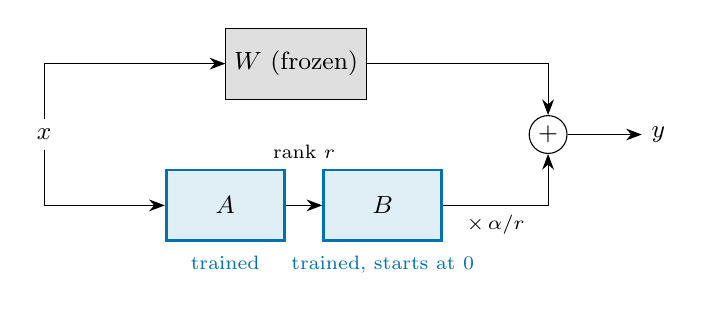
\begin{tikzpicture}[font=\small, >={Stealth[length=2mm]},
  box/.style={draw, minimum height=0.9cm, minimum width=1.5cm, inner sep=3pt}]
  \node (x) at (0,0) {$x$};
  \node[box, fill=cGrey!25] (W) at (3.2,0.9) {$W$ (frozen)};
  \node[box, draw=cAttn, line width=1pt, fill=cAttn!12] (A) at (2.3,-0.9) {$A$};
  \node[box, draw=cAttn, line width=1pt, fill=cAttn!12] (B) at (4.3,-0.9) {$B$};
  \node[draw, circle, inner sep=1.5pt] (p) at (6.4,0) {$+$};
  \node (y) at (7.8,0) {$y$};
  \draw[->] (x) |- (W);
  \draw[->] (x) |- (A);
  \draw[->] (A) -- (B);
  \node[font=\scriptsize] at (3.3,-0.22) {rank $r$};
  \draw[->] (W) -| (p);
  \draw[->] (B) -| node[pos=0.25, below, font=\scriptsize] {$\times\,\alpha/r$} (p);
  \draw[->] (p) -- (y);
  \node[font=\scriptsize, text=cAttn, below=0.05cm of A] {trained};
  \node[font=\scriptsize, text=cAttn, below=0.05cm of B] {trained, starts at 0};
\end{tikzpicture}
}
\par\medskip\small
\begin{enumerate}
  \item Is it as \textbf{accurate}?
  \item What does it save in \textbf{training}?
  \item \textbf{Where} should the adapters go?
  \item What changes at \textbf{deployment}?
\end{enumerate}
\end{column}
\end{columns}
\end{frame}

% 3 ---------------------------------------------------------------------------------------------------------------
\subsection{3. Setup: two models, the same configurations, five seeds}
\begin{frame}{Setup: two models, the same configurations, five seeds}
\begin{columns}[T]
\begin{column}{0.5\textwidth}
\small
\begin{tabular}{@{}ll@{}}
\toprule
models & ViT-B/16 (12 equal blocks)\\
 & Swin-B (24 blocks, 4 stages)\\
data & CIFAR-100, upsampled to 224\\
 & 45k train / 5k validation / 10k test\\
full FT & all weights; rate chosen on\\
 & validation loss ($3{\times}10^{-5}$, $10^{-5}$)\\
LoRA & rank 8, rate $10^{-4}$\\
 & on attention, MLP, or both\\
training & batch 64, early stopping\\
seeds & 5 per configuration\\
\bottomrule
\end{tabular}
\end{column}
\begin{column}{0.47\textwidth}
\small
\textbf{How we compare}
\begin{itemize}
  \item mean $\pm$ standard deviation over seeds
  \item \textbf{paired difference}: seed by seed, then averaged
  \item for each difference: in how many seeds it goes the same way (e.g.\ LoRA ahead in 5 of 5 seeds)
  \item times are compared \textbf{per epoch}
\end{itemize}
\medskip
Every comparison uses the same configurations and seeds on both models.
\end{column}
\end{columns}
\end{frame}

% 4 ---------------------------------------------------------------------------------------------------------------
\subsection{4. Full fine-tuning must be tuned before it is compared}
\begin{frame}{Full fine-tuning must be tuned before it is compared}
\vspace{-1mm}
{\renewcommand{\figH}{4.2cm}\centering% generated by scripts/make_figures.py; do not edit
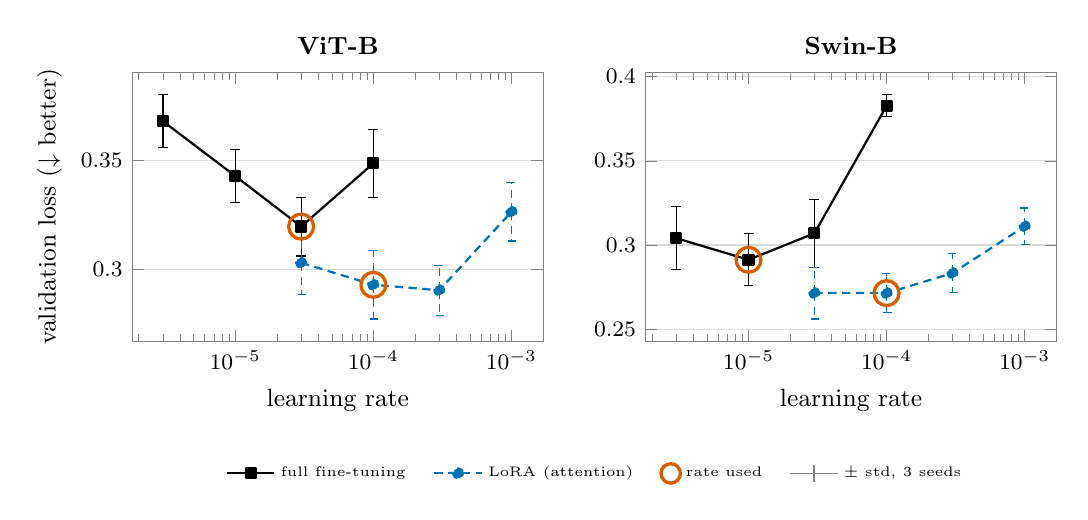
\begin{tikzpicture}
\begin{groupplot}[group style={group size=2 by 1, horizontal sep=\figSep, vertical sep=1.3cm}, width=\figW, height=\figH, repaxis, xmode=log, xmin=1.8e-6, xmax=1.7e-3, ymajorgrids, xlabel={learning rate}, legend style={font=\figLegendFont, draw=none, fill=none, at={(-0.12,-0.42)}, anchor=north, legend columns=-1, /tikz/every even column/.append style={column sep=8pt}}]
\nextgroupplot[title={ViT-B}, ylabel={validation loss ($\downarrow$ better)}, ylabel style={align=center}]
\addplot[cFT, solid, thick, mark=square*, mark size=1.8pt, forget plot, error bars/.cd, y dir=both, y explicit] coordinates {(3e-06,0.3681) +- (0,0.0122) (1e-05,0.3430) +- (0,0.0122) (3e-05,0.3198) +- (0,0.0135) (0.0001,0.3488) +- (0,0.0156)};
\addplot[cAccent, only marks, mark=o, mark size=4.5pt, very thick, forget plot] coordinates {(3e-05,0.3198)};
\addplot[cAttn, densely dashed, thick, mark=*, mark size=1.8pt, forget plot, error bars/.cd, y dir=both, y explicit] coordinates {(3e-05,0.3032) +- (0,0.0144) (0.0001,0.2931) +- (0,0.0157) (0.0003,0.2906) +- (0,0.0115) (0.001,0.3266) +- (0,0.0134)};
\addplot[cAccent, only marks, mark=o, mark size=4.5pt, very thick, forget plot] coordinates {(0.0001,0.2931)};
\nextgroupplot[title={Swin-B}]
\addplot[cFT, solid, thick, mark=square*, mark size=1.8pt, forget plot, error bars/.cd, y dir=both, y explicit] coordinates {(3e-06,0.3040) +- (0,0.0188) (1e-05,0.2912) +- (0,0.0155) (3e-05,0.3069) +- (0,0.0203) (0.0001,0.3827) +- (0,0.0066)};
\addplot[cAccent, only marks, mark=o, mark size=4.5pt, very thick, forget plot] coordinates {(1e-05,0.2912)};
\addplot[cAttn, densely dashed, thick, mark=*, mark size=1.8pt, forget plot, error bars/.cd, y dir=both, y explicit] coordinates {(3e-05,0.2714) +- (0,0.0154) (0.0001,0.2714) +- (0,0.0115) (0.0003,0.2833) +- (0,0.0114) (0.001,0.3111) +- (0,0.0109)};
\addplot[cAccent, only marks, mark=o, mark size=4.5pt, very thick, forget plot] coordinates {(0.0001,0.2714)};
\addlegendimage{cFT, solid, thick, mark=square*, mark size=1.8pt}
\addlegendentry{full fine-tuning}
\addlegendimage{cAttn, densely dashed, thick, mark=*, mark size=1.8pt}
\addlegendentry{LoRA (attention)}
\addlegendimage{cAccent, only marks, mark=o, mark size=3.5pt, very thick}
\addlegendentry{rate used}
\addlegendimage{cGrey, mark=|, mark size=3pt}
\addlegendentry{$\pm$ std, 3 seeds}
\end{groupplot}
\end{tikzpicture}
\par}
\vspace{-1mm}
\begin{columns}[T]
\begin{column}{0.48\textwidth}
\footnotesize
\begin{itemize}
  \item four rates per method, 3 seeds; the best rate is the one with the lowest validation loss
  \item full fine-tuning: \textbf{$3{\times}10^{-5}$ on ViT-B}, \textbf{$10^{-5}$ on Swin-B}; worse on both sides
\end{itemize}
\end{column}
\begin{column}{0.48\textwidth}
\footnotesize
\begin{itemize}
  \item LoRA: $10^{-4}$ is at, or tied with, its best rate on both models
  \item ViT-B full fine-tuning at $10^{-5}$ instead of $3{\times}10^{-5}$: \textbf{0.6 pp} less accurate, enough to make LoRA look better
\end{itemize}
\end{column}
\end{columns}
\src{Validation loss of the tested weights (lower is better); error bars: std over 3 seeds. The 0.6 pp: 5 seeds. All numbers: backup slide.}
\end{frame}

% 5 ---------------------------------------------------------------------------------------------------------------
\subsection{5. LoRA is ahead on Swin-B; on ViT-B it is level or slightly behind}
\begin{frame}{LoRA is ahead on Swin-B; on ViT-B it is level or slightly behind}
\vspace{-1mm}
{\renewcommand{\figH}{4.5cm}\centering% generated by scripts/make_figures.py; do not edit
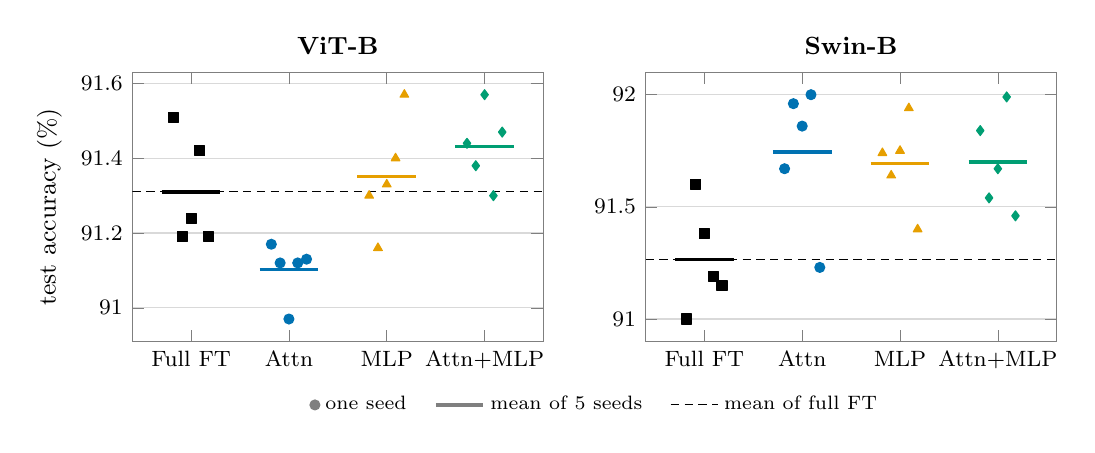
\begin{tikzpicture}
\begin{groupplot}[group style={group size=2 by 1, horizontal sep=\figSep, vertical sep=1.3cm}, width=\figW, height=\figH, repaxis, xmin=0.4, xmax=4.6, xtick={1,2,3,4}, xticklabels={Full FT,Attn,MLP,Attn+MLP}, ymajorgrids, legend style={font=\scriptsize, draw=none, fill=none, at={(-0.12,-0.16)}, anchor=north, legend columns=-1, /tikz/every even column/.append style={column sep=8pt}}]
\nextgroupplot[title={ViT-B}, ylabel={test accuracy (\%)}]
\addplot[only marks, mark=square*, mark size=1.8pt, cFT, forget plot] coordinates {(0.82,91.51) (0.91,91.19) (1.00,91.24) (1.09,91.42) (1.18,91.19)};
\draw[cFT, line width=1.2pt] (axis cs:0.7,91.310) -- (axis cs:1.3,91.310);
\addplot[only marks, mark=*, mark size=1.8pt, cAttn, forget plot] coordinates {(1.82,91.17) (1.91,91.12) (2.00,90.97) (2.09,91.12) (2.18,91.13)};
\draw[cAttn, line width=1.2pt] (axis cs:1.7,91.102) -- (axis cs:2.3,91.102);
\addplot[only marks, mark=triangle*, mark size=1.8pt, cMLP, forget plot] coordinates {(2.82,91.30) (2.91,91.16) (3.00,91.33) (3.09,91.40) (3.18,91.57)};
\draw[cMLP, line width=1.2pt] (axis cs:2.7,91.352) -- (axis cs:3.3,91.352);
\addplot[only marks, mark=diamond*, mark size=1.8pt, cBoth, forget plot] coordinates {(3.82,91.44) (3.91,91.38) (4.00,91.57) (4.09,91.30) (4.18,91.47)};
\draw[cBoth, line width=1.2pt] (axis cs:3.7,91.432) -- (axis cs:4.3,91.432);
\draw[cFT, densely dashed] (axis cs:0.4,91.310) -- (axis cs:4.6,91.310);
\nextgroupplot[title={Swin-B}]
\addplot[only marks, mark=square*, mark size=1.8pt, cFT, forget plot] coordinates {(0.82,91.00) (0.91,91.60) (1.00,91.38) (1.09,91.19) (1.18,91.15)};
\draw[cFT, line width=1.2pt] (axis cs:0.7,91.264) -- (axis cs:1.3,91.264);
\addplot[only marks, mark=*, mark size=1.8pt, cAttn, forget plot] coordinates {(1.82,91.67) (1.91,91.96) (2.00,91.86) (2.09,92.00) (2.18,91.23)};
\draw[cAttn, line width=1.2pt] (axis cs:1.7,91.744) -- (axis cs:2.3,91.744);
\addplot[only marks, mark=triangle*, mark size=1.8pt, cMLP, forget plot] coordinates {(2.82,91.74) (2.91,91.64) (3.00,91.75) (3.09,91.94) (3.18,91.40)};
\draw[cMLP, line width=1.2pt] (axis cs:2.7,91.694) -- (axis cs:3.3,91.694);
\addplot[only marks, mark=diamond*, mark size=1.8pt, cBoth, forget plot] coordinates {(3.82,91.84) (3.91,91.54) (4.00,91.67) (4.09,91.99) (4.18,91.46)};
\draw[cBoth, line width=1.2pt] (axis cs:3.7,91.700) -- (axis cs:4.3,91.700);
\draw[cFT, densely dashed] (axis cs:0.4,91.264) -- (axis cs:4.6,91.264);
\addlegendimage{only marks, mark=*, mark size=1.8pt, cGrey}
\addlegendentry{one seed}
\addlegendimage{cGrey, line width=1.2pt}
\addlegendentry{mean of 5 seeds}
\addlegendimage{cFT, densely dashed}
\addlegendentry{mean of full FT}
\end{groupplot}
\end{tikzpicture}
\par}
\vspace{1mm}
\vspace{-1mm}
\begin{columns}[T]
\begin{column}{0.48\textwidth}
\footnotesize
\begin{itemize}
  \item \textbf{ViT-B}: MLP $+$0.04, Attn+MLP $+$0.12 pp (within the spread over seeds); attention \textbf{$-$0.21 $\pm$ 0.13 pp}, lower in 5 of 5 seeds
  \item training the same configuration again moved its mean by 0.2 pp, as much as this gap
\end{itemize}
\end{column}
\begin{column}{0.48\textwidth}
\footnotesize
\begin{itemize}
  \item \textbf{Swin-B}: $+$0.43 to $+$0.48 pp, ahead in \textbf{5, 5 and 4 of 5} seeds
\end{itemize}
\end{column}
\end{columns}
\src{LoRA rank 8 on all blocks, rate $10^{-4}$; full fine-tuning at its best rate; 5 seeds.}
\end{frame}

% 6 ---------------------------------------------------------------------------------------------------------------
\subsection{6. Training memory: the saving depends on which layers are adapted}
\begin{frame}{Training memory: the saving depends on which layers are adapted}
\vspace{-1mm}
{\centering% generated by scripts/make_figures.py; do not edit
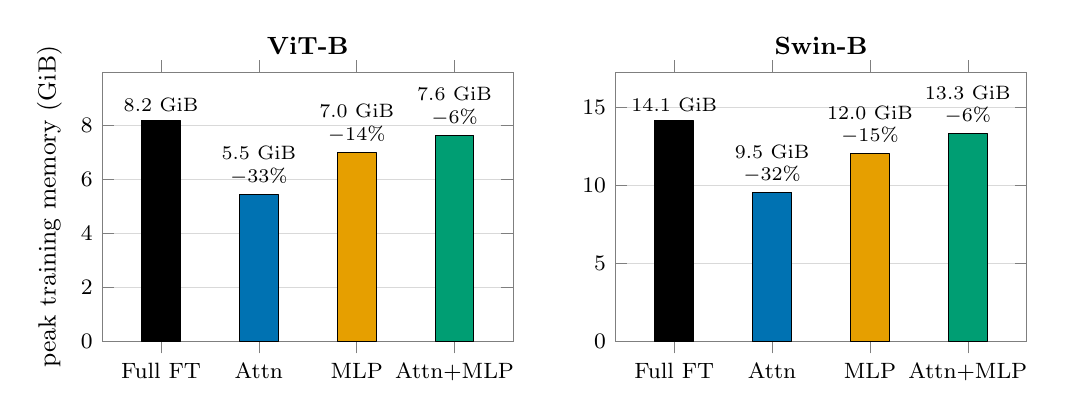
\begin{tikzpicture}
\begin{groupplot}[group style={group size=2 by 1, horizontal sep=\figSep, vertical sep=1.3cm}, width=\figW, height=\figH, repaxis, ybar, /pgf/bar width=14pt, xmin=0.4, xmax=4.6, ymin=0, xtick={1,2,3,4}, xticklabels={Full FT,Attn,MLP,Attn+MLP}, ymajorgrids, enlarge y limits={upper, value=0.22}]
\nextgroupplot[title={ViT-B}, ylabel={peak training memory (GiB)}]
\addplot[fill=cFT, draw=black, bar shift=0pt] coordinates {(1,8.174)};
\node[font=\scriptsize, anchor=south, align=center] at (axis cs:1,8.174) {8.2 GiB};
\addplot[fill=cAttn, draw=black, bar shift=0pt] coordinates {(2,5.459)};
\node[font=\scriptsize, anchor=south, align=center] at (axis cs:2,5.459) {5.5 GiB\\$-$33\%};
\addplot[fill=cMLP, draw=black, bar shift=0pt] coordinates {(3,7.011)};
\node[font=\scriptsize, anchor=south, align=center] at (axis cs:3,7.011) {7.0 GiB\\$-$14\%};
\addplot[fill=cBoth, draw=black, bar shift=0pt] coordinates {(4,7.643)};
\node[font=\scriptsize, anchor=south, align=center] at (axis cs:4,7.643) {7.6 GiB\\$-$6\%};
\nextgroupplot[title={Swin-B}]
\addplot[fill=cFT, draw=black, bar shift=0pt] coordinates {(1,14.121)};
\node[font=\scriptsize, anchor=south, align=center] at (axis cs:1,14.121) {14.1 GiB};
\addplot[fill=cAttn, draw=black, bar shift=0pt] coordinates {(2,9.549)};
\node[font=\scriptsize, anchor=south, align=center] at (axis cs:2,9.549) {9.5 GiB\\$-$32\%};
\addplot[fill=cMLP, draw=black, bar shift=0pt] coordinates {(3,12.007)};
\node[font=\scriptsize, anchor=south, align=center] at (axis cs:3,12.007) {12.0 GiB\\$-$15\%};
\addplot[fill=cBoth, draw=black, bar shift=0pt] coordinates {(4,13.290)};
\node[font=\scriptsize, anchor=south, align=center] at (axis cs:4,13.290) {13.3 GiB\\$-$6\%};
\end{groupplot}
\end{tikzpicture}
\par}
\vspace{-1mm}
\begin{columns}[T]
\begin{column}{0.48\textwidth}
\footnotesize
\begin{itemize}
  \item attention: \textbf{a third} less
  \item MLP: a seventh less; both: about 6\% less
\end{itemize}
\end{column}
\begin{column}{0.48\textwidth}
\footnotesize
\take{The same pattern on both models.}
Peak memory at batch size 64; identical in all 5 seeds.
\end{column}
\end{columns}
\end{frame}

% 7 ---------------------------------------------------------------------------------------------------------------
\subsection{7. Why: memory is what the backward pass must keep}
\begin{frame}{Why: memory is what the backward pass must keep}
\centering
\scalebox{0.95}{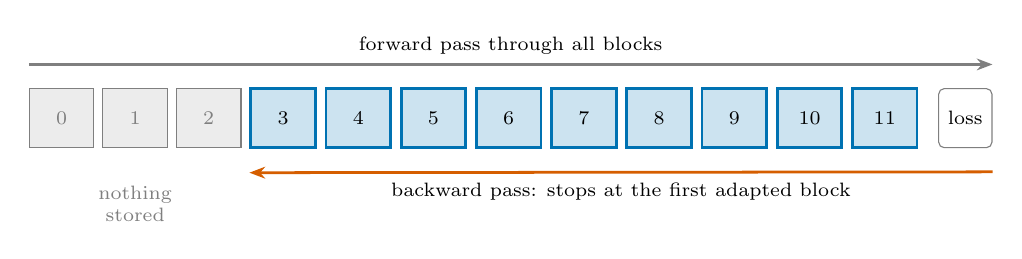
\begin{tikzpicture}[>={Stealth[length=2mm]},
  blk/.style={draw=cGrey, minimum width=0.82cm, minimum height=0.75cm, font=\scriptsize, inner sep=1pt},
  fwd/.style={blk, fill=cGrey!15, text=cGrey},
  ad/.style={blk, draw=cAttn, line width=1pt, fill=cAttn!20}]
  \node[fwd] (b0) at (0,0) {0};
  \foreach \i/\j in {1/0,2/1} {\node[fwd, right=0.1cm of b\j] (b\i) {\i};}
  \foreach \i/\j in {3/2,4/3,5/4,6/5,7/6,8/7,9/8,10/9,11/10} {\node[ad, right=0.1cm of b\j] (b\i) {\i};}
  \node[draw=cGrey, rounded corners=2pt, font=\scriptsize, right=0.25cm of b11, minimum height=0.75cm] (loss) {loss};
  \draw[->, cGrey, line width=0.8pt] ($(b0.north west)+(0,0.3)$) -- node[above, font=\scriptsize, text=black] {forward pass through all blocks} ($(loss.north east)+(0,0.3)$);
  \draw[->, cAccent, line width=1pt] ($(loss.south east)+(0,-0.3)$) -- node[below, font=\scriptsize, text=black] {backward pass: stops at the first adapted block} ($(b3.south west)+(0,-0.3)$);
  \node[font=\scriptsize, text=cGrey, align=center, below=0.35cm of b1] {nothing\\stored};
\end{tikzpicture}
}
\par\medskip
\begin{columns}[T]
\begin{column}{0.47\textwidth}
\small
\begin{itemize}
  \item Only 1.3 of the 8.2 GiB of full fine-tuning is weights and optimiser state (ViT-B); the rest is kept activations
  \item A \textbf{frozen linear layer} keeps nothing (normalisation, GELU and attention still do)
  \item An \textbf{adapter} needs the input of its layer
\end{itemize}
\end{column}
\begin{column}{0.5\textwidth}
\small
\begin{itemize}
  \item The MLP's hidden layer is $4\times$ wider, so MLP adapters keep much more
  \item Blocks \textbf{before the first adapter} keep nothing at all
\end{itemize}
\take{Trained parameters do not predict training memory.}
\end{column}
\end{columns}
\end{frame}

% 8 ---------------------------------------------------------------------------------------------------------------
\subsection{8. The saving is largest at small batches}
\begin{frame}{The saving is largest at small batches}
\vspace{-1mm}
{\centering% generated by scripts/make_figures.py; do not edit
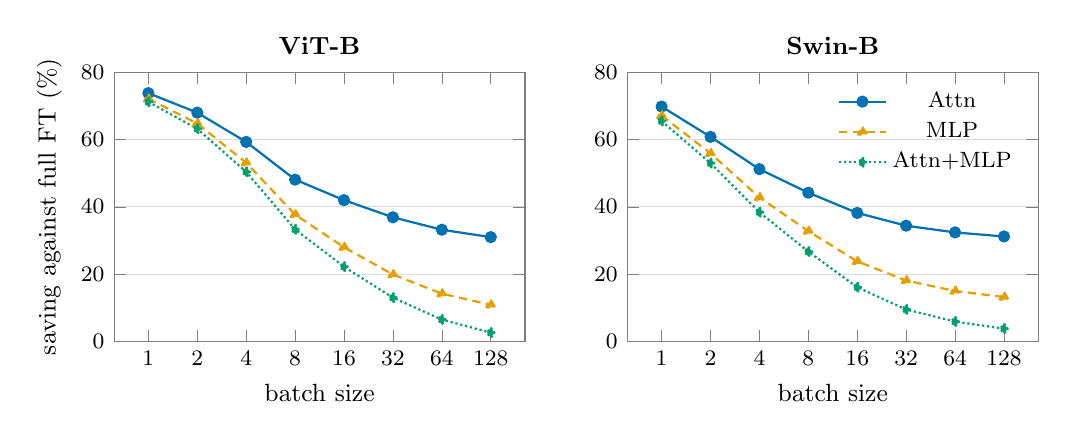
\begin{tikzpicture}
\begin{groupplot}[group style={group size=2 by 1, horizontal sep=\figSep, vertical sep=1.3cm}, width=\figW, height=\figH, repaxis, xmode=log, log basis x=2, xtick={1,2,4,8,16,32,64,128}, xticklabels={1,2,4,8,16,32,64,128}, ymin=0, ymax=80, ymajorgrids, legend style={font=\footnotesize, draw=none, fill=none}, legend pos=north east]
\nextgroupplot[title={ViT-B}, xlabel={batch size}, ylabel={saving against full FT (\%)}]
\addplot[cAttn, solid, thick, mark=*, mark size=1.8pt] coordinates {(1,73.8) (2,68.0) (4,59.3) (8,48.1) (16,42.0) (32,36.9) (64,33.2) (128,31.0)};
\addplot[cMLP, densely dashed, thick, mark=triangle*, mark size=1.8pt] coordinates {(1,72.1) (2,64.8) (4,53.1) (8,37.7) (16,28.0) (32,19.9) (64,14.2) (128,10.9)};
\addplot[cBoth, densely dotted, thick, mark=diamond*, mark size=1.8pt] coordinates {(1,71.2) (2,63.2) (4,50.4) (8,33.3) (16,22.2) (32,13.0) (64,6.5) (128,2.6)};
\nextgroupplot[title={Swin-B}, xlabel={batch size}]
\addplot[cAttn, solid, thick, mark=*, mark size=1.8pt] coordinates {(1,69.8) (2,60.8) (4,51.2) (8,44.2) (16,38.2) (32,34.4) (64,32.4) (128,31.2)};
\addlegendentry{Attn}
\addplot[cMLP, densely dashed, thick, mark=triangle*, mark size=1.8pt] coordinates {(1,67.1) (2,55.9) (4,42.8) (8,32.8) (16,23.8) (32,18.1) (64,15.0) (128,13.2)};
\addlegendentry{MLP}
\addplot[cBoth, densely dotted, thick, mark=diamond*, mark size=1.8pt] coordinates {(1,65.5) (2,53.0) (4,38.4) (8,26.7) (16,16.1) (32,9.5) (64,5.9) (128,3.8)};
\addlegendentry{Attn+MLP}
\end{groupplot}
\end{tikzpicture}
\par}
\vspace{-1mm}
\begin{columns}[T]
\begin{column}{0.48\textwidth}
\footnotesize
\begin{itemize}
  \item batch 1: \textbf{66--74\%} less memory for every target
  \item batch 128: 31\% (attention), 11--13\% (MLP), 3--4\% (both)
\end{itemize}
\end{column}
\begin{column}{0.48\textwidth}
\footnotesize
\take{Small batches are where memory-limited devices work.}
\end{column}
\end{columns}
\src{Peak memory of one training step (profiler). Full fine-tuning of Swin-B does not fit at batch 256.}
\end{frame}

% 9 --------------------------------------------------------------------------------------------------------------
\subsection{9. Training is faster per epoch, and a task is stored in megabytes}
\begin{frame}{Training is faster per epoch, and a task is stored in megabytes}
\vspace{-1mm}
{\centering% generated by scripts/make_figures.py; do not edit
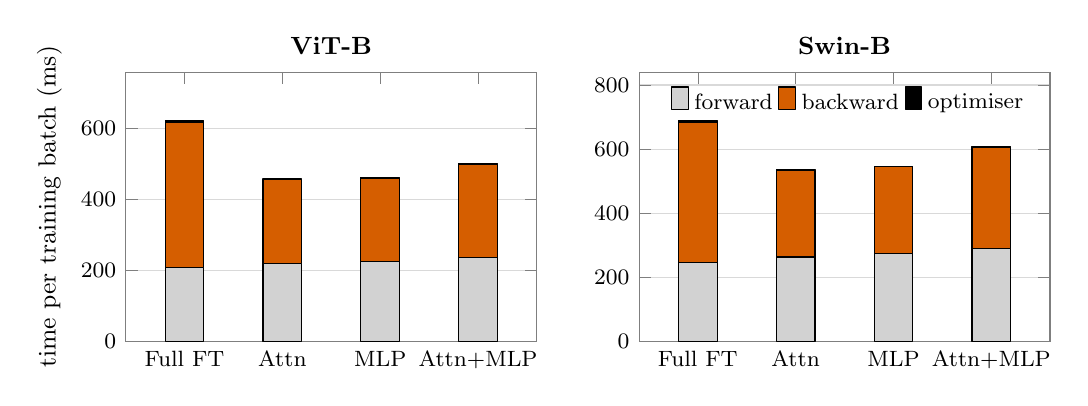
\begin{tikzpicture}
\begin{groupplot}[group style={group size=2 by 1, horizontal sep=\figSep, vertical sep=1.3cm}, width=\figW, height=\figH, repaxis, ybar stacked, /pgf/bar width=14pt, xmin=0.4, xmax=4.6, ymin=0, xtick={1,2,3,4}, xticklabels={Full FT,Attn,MLP,Attn+MLP}, ymajorgrids, legend style={font=\footnotesize, draw=none, fill=none}, legend pos=north east, legend columns=-1, enlarge y limits={upper, value=0.22}]
\nextgroupplot[title={ViT-B}, ylabel={time per training batch (ms)}]
\addplot[fill=cGrey!35, draw=black] coordinates {(1,208.6) (2,219.8) (3,224.9) (4,235.5)};
\addplot[fill=cAccent, draw=black] coordinates {(1,407.9) (2,236.9) (3,235.1) (4,264.0)};
\addplot[fill=black, draw=black] coordinates {(1,5.5) (2,1.1) (3,1.0) (4,1.6)};
\nextgroupplot[title={Swin-B}]
\addplot[fill=cGrey!35, draw=black] coordinates {(1,245.8) (2,263.4) (3,273.4) (4,289.9)};
\addlegendentry{forward}
\addplot[fill=cAccent, draw=black] coordinates {(1,435.9) (2,271.1) (3,271.6) (4,315.4)};
\addlegendentry{backward}
\addplot[fill=black, draw=black] coordinates {(1,6.5) (2,1.4) (3,1.1) (4,2.2)};
\addlegendentry{optimiser}
\end{groupplot}
\end{tikzpicture}
\par}
\vspace{-1mm}
\begin{columns}[T]
\begin{column}{0.48\textwidth}
\footnotesize
\begin{itemize}
  \item train epoch: \textbf{19--26\%} shorter (ViT-B), \textbf{12--22\%} (Swin-B)
  \item backward pass and optimiser get cheaper; the forward pass gets slightly slower
\end{itemize}
\end{column}
\begin{column}{0.48\textwidth}
\footnotesize
\begin{itemize}
  \item stored per task: \textbf{2--6 MiB} instead of 330 MiB
  \item this helps only when tasks share one base model
\end{itemize}
\end{column}
\end{columns}
\end{frame}

% 10 --------------------------------------------------------------------------------------------------------------
\subsection{10. Placement: adapting only the second half costs accuracy}
\begin{frame}{Placement: adapting only the second half costs accuracy}
\vspace{-1mm}
{\renewcommand{\figH}{3.8cm}\centering% generated by scripts/make_figures.py; do not edit
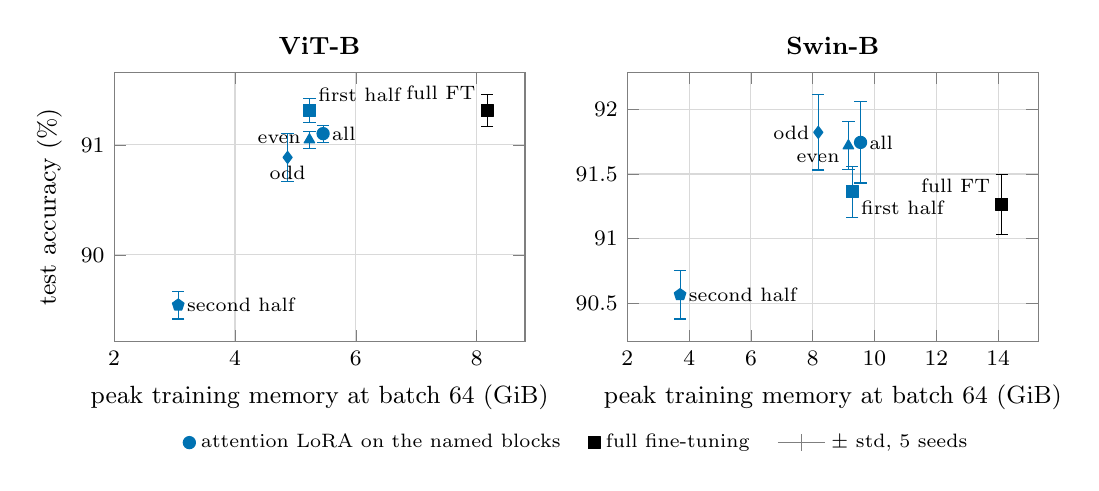
\begin{tikzpicture}
\begin{groupplot}[group style={group size=2 by 1, horizontal sep=\figSep, vertical sep=1.3cm}, width=\figW, height=\figH, repaxis, ymajorgrids, xmajorgrids, xlabel={peak training memory at batch 64 (GiB)}, legend style={font=\scriptsize, draw=none, fill=none, at={(-0.12,-0.3)}, anchor=north, legend columns=-1, /tikz/every even column/.append style={column sep=8pt}}]
\nextgroupplot[title={ViT-B}, xmin=2, xmax=8.8, ylabel={test accuracy (\%)}]
\addplot[cAttn, only marks, mark=*, mark size=2.2pt, forget plot, error bars/.cd, y dir=both, y explicit] coordinates {(5.459,91.102) +- (0,0.077)};
\node[font=\scriptsize, anchor=west, inner sep=3pt] at (axis cs:5.459,91.102) {all};
\addplot[cAttn, only marks, mark=square*, mark size=2.2pt, forget plot, error bars/.cd, y dir=both, y explicit] coordinates {(5.233,91.314) +- (0,0.109)};
\node[font=\scriptsize, anchor=south west, inner sep=3pt] at (axis cs:5.233,91.314) {first half};
\addplot[cAttn, only marks, mark=triangle*, mark size=2.2pt, forget plot, error bars/.cd, y dir=both, y explicit] coordinates {(5.233,91.046) +- (0,0.075)};
\node[font=\scriptsize, anchor=east, inner sep=3pt] at (axis cs:5.233,91.046) {even};
\addplot[cAttn, only marks, mark=diamond*, mark size=2.2pt, forget plot, error bars/.cd, y dir=both, y explicit] coordinates {(4.871,90.886) +- (0,0.215)};
\node[font=\scriptsize, anchor=north, inner sep=3pt] at (axis cs:4.871,90.886) {odd};
\addplot[cAttn, only marks, mark=pentagon*, mark size=2.2pt, forget plot, error bars/.cd, y dir=both, y explicit] coordinates {(3.061,89.544) +- (0,0.127)};
\node[font=\scriptsize, anchor=west, inner sep=3pt] at (axis cs:3.061,89.544) {second half};
\addplot[cFT, only marks, mark=square*, mark size=2.2pt, forget plot, error bars/.cd, y dir=both, y explicit] coordinates {(8.174,91.310) +- (0,0.146)};
\node[font=\scriptsize, anchor=south east, inner sep=4pt] at (axis cs:8.174,91.310) {full FT};
\nextgroupplot[title={Swin-B}, xmin=2, xmax=15.3]
\addplot[cAttn, only marks, mark=*, mark size=2.2pt, forget plot, error bars/.cd, y dir=both, y explicit] coordinates {(9.549,91.744) +- (0,0.314)};
\node[font=\scriptsize, anchor=west, inner sep=3pt] at (axis cs:9.549,91.744) {all};
\addplot[cAttn, only marks, mark=square*, mark size=2.2pt, forget plot, error bars/.cd, y dir=both, y explicit] coordinates {(9.284,91.362) +- (0,0.197)};
\node[font=\scriptsize, anchor=north west, inner sep=3pt] at (axis cs:9.284,91.362) {first half};
\addplot[cAttn, only marks, mark=triangle*, mark size=2.2pt, forget plot, error bars/.cd, y dir=both, y explicit] coordinates {(9.156,91.718) +- (0,0.186)};
\node[font=\scriptsize, anchor=north east, inner sep=3pt] at (axis cs:9.156,91.718) {even};
\addplot[cAttn, only marks, mark=diamond*, mark size=2.2pt, forget plot, error bars/.cd, y dir=both, y explicit] coordinates {(8.180,91.822) +- (0,0.291)};
\node[font=\scriptsize, anchor=east, inner sep=3pt] at (axis cs:8.180,91.822) {odd};
\addplot[cAttn, only marks, mark=pentagon*, mark size=2.2pt, forget plot, error bars/.cd, y dir=both, y explicit] coordinates {(3.707,90.566) +- (0,0.188)};
\node[font=\scriptsize, anchor=west, inner sep=3pt] at (axis cs:3.707,90.566) {second half};
\addplot[cFT, only marks, mark=square*, mark size=2.2pt, forget plot, error bars/.cd, y dir=both, y explicit] coordinates {(14.121,91.264) +- (0,0.232)};
\node[font=\scriptsize, anchor=south east, inner sep=4pt] at (axis cs:14.121,91.264) {full FT};
\addlegendimage{cAttn, only marks, mark=*, mark size=2.2pt}
\addlegendentry{attention LoRA on the named blocks}
\addlegendimage{cFT, only marks, mark=square*, mark size=2.2pt}
\addlegendentry{full fine-tuning}
\addlegendimage{cGrey, mark=|, mark size=3pt}
\addlegendentry{$\pm$ std, 5 seeds}
\end{groupplot}
\end{tikzpicture}
\par}
\vspace{-2mm}
\begin{columns}[T]
\begin{column}{0.48\textwidth}
\footnotesize
\begin{itemize}
  \item \textbf{second half}: $-$1.56 pp (ViT-B), $-$1.18 pp (Swin-B), lower in \textbf{all 5 seeds}; below full FT on both
  \item \textbf{first half}: $+$0.21 pp on ViT-B, higher in all 5 seeds; $-$0.38 pp on Swin-B, lower in all 5
\end{itemize}
\end{column}
\begin{column}{0.48\textwidth}
\footnotesize
\take{Later half only: 1.2--1.6 pp less accurate, below full FT on both models.}
The pp values on the left: change against attention LoRA on all blocks, compared seed by seed.
\end{column}
\end{columns}
\end{frame}

% 11 --------------------------------------------------------------------------------------------------------------
\subsection{11. Training memory is set by the first adapted block}
\begin{frame}{Training memory is set by the first adapted block}
\vspace{-1mm}
{\renewcommand{\figH}{4.4cm}\centering% generated by scripts/make_figures.py; do not edit
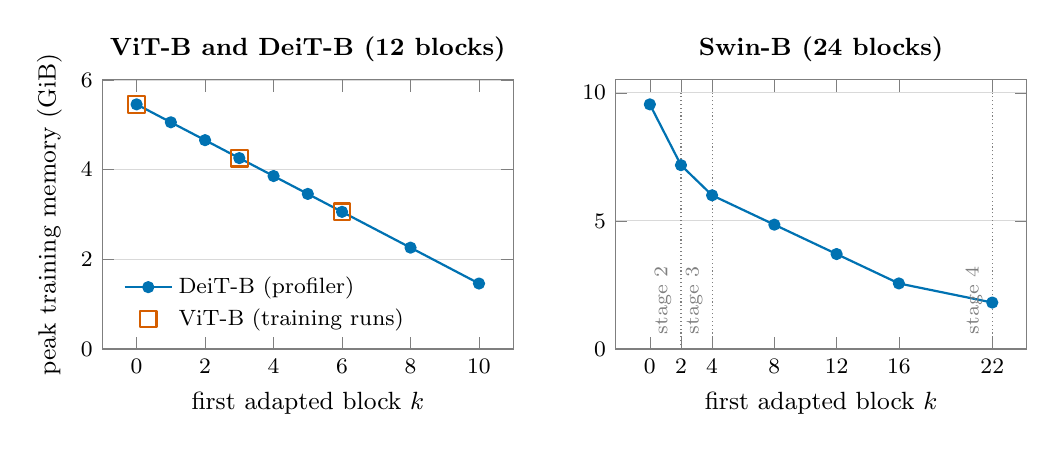
\begin{tikzpicture}
\begin{groupplot}[group style={group size=2 by 1, horizontal sep=\figSep, vertical sep=1.3cm}, width=\figW, height=\figH, repaxis, ymin=0, ymajorgrids, xlabel={first adapted block $k$}, legend style={font=\footnotesize, draw=none, fill=none, legend cell align=left}, legend pos=south west]
\nextgroupplot[title={ViT-B and DeiT-B (12 blocks)}, ylabel={peak training memory (GiB)}, xtick={0,2,4,6,8,10}]
\addplot[cAttn, thick, mark=*, mark size=1.8pt] coordinates {(0,5.459) (1,5.059) (2,4.660) (3,4.260) (4,3.860) (5,3.461) (6,3.061) (8,2.262) (10,1.462)};
\addlegendentry{DeiT-B (profiler)}
\addplot[cAccent, only marks, mark=square, mark size=3pt, thick] coordinates {(0,5.459) (3,4.260) (6,3.061)};
\addlegendentry{ViT-B (training runs)}
\nextgroupplot[title={Swin-B (24 blocks)}, xtick={0,2,4,8,12,16,22}]
\addplot[cAttn, thick, mark=*, mark size=1.8pt] coordinates {(0,9.549) (2,7.175) (4,6.000) (8,4.854) (12,3.707) (16,2.560) (22,1.815)};
\draw[cGrey, densely dotted] (axis cs:2,0) -- (axis cs:2,10);
\node[font=\scriptsize, cGrey, rotate=90, anchor=south west] at (axis cs:2,0.2) {stage 2};
\draw[cGrey, densely dotted] (axis cs:4,0) -- (axis cs:4,10);
\node[font=\scriptsize, cGrey, rotate=90, anchor=south west] at (axis cs:4,0.2) {stage 3};
\draw[cGrey, densely dotted] (axis cs:22,0) -- (axis cs:22,10);
\node[font=\scriptsize, cGrey, rotate=90, anchor=south west] at (axis cs:22,0.2) {stage 4};
\end{groupplot}
\end{tikzpicture}
\par}
\vspace{-1mm}
\begin{columns}[T]
\begin{column}{0.48\textwidth}
\footnotesize
\begin{itemize}
  \item ViT-B: first half $=$ even blocks $=$ 5.233 GiB (both start at block 0)
  \item each block later that the adapters start saves \textbf{0.40 GiB}
\end{itemize}
\end{column}
\begin{column}{0.48\textwidth}
\footnotesize
\begin{itemize}
  \item Swin-B: block 0 alone is \textbf{0.98 GiB}
  \item one more adapted block after the start: only 0.04 GiB
\end{itemize}
\end{column}
\end{columns}
\src{Attention LoRA on every block from $k$ to the last, batch 64. ViT-B odd blocks and second half: same trainable parameters, 1.81 GiB apart.}
\end{frame}

% 12 --------------------------------------------------------------------------------------------------------------
\subsection{12. Deployment: a merged LoRA model is an ordinary model}
\begin{frame}{Deployment: a merged LoRA model is an ordinary model}
\begin{columns}[T]
\begin{column}{0.47\textwidth}
\small
\textbf{Merging changes nothing} (7 configurations per model)
\begin{itemize}
  \item same class on 10,000 of 10,000 test images
  \item outputs equal up to rounding ($\le 5\times10^{-6}$)
  \item still exact after 100 merge/unmerge cycles
\end{itemize}
\medskip
\textbf{Speed}: merged $=$ dense\\
7.13--7.15 vs 7.12 ms (ViT-B)\\ 9.75--9.92 vs 9.74 ms (Swin-B)
\end{column}
\begin{column}{0.5\textwidth}
\small
\textbf{Inference memory} at batch 64 (GiB)\par\smallskip
\begin{tabular}{@{}lcc@{}}
\toprule
 & ViT-B & Swin-B \\
\midrule
dense & 0.799 & 1.805 \\
merged LoRA & 0.799 & 1.805 \\
unmerged, attention & 0.801 & 1.807 \\
unmerged, MLP & 0.946 & 2.192 \\
\bottomrule
\end{tabular}
\take{LoRA does not make inference cheaper. Its saving is in training.}
\end{column}
\end{columns}
\end{frame}

% 13 --------------------------------------------------------------------------------------------------------------
\subsection{13. Unmerged adapters slow down single-image predictions}
\begin{frame}{Unmerged adapters slow down single-image predictions}
\vspace{-1mm}
{\centering% generated by scripts/make_figures.py; do not edit
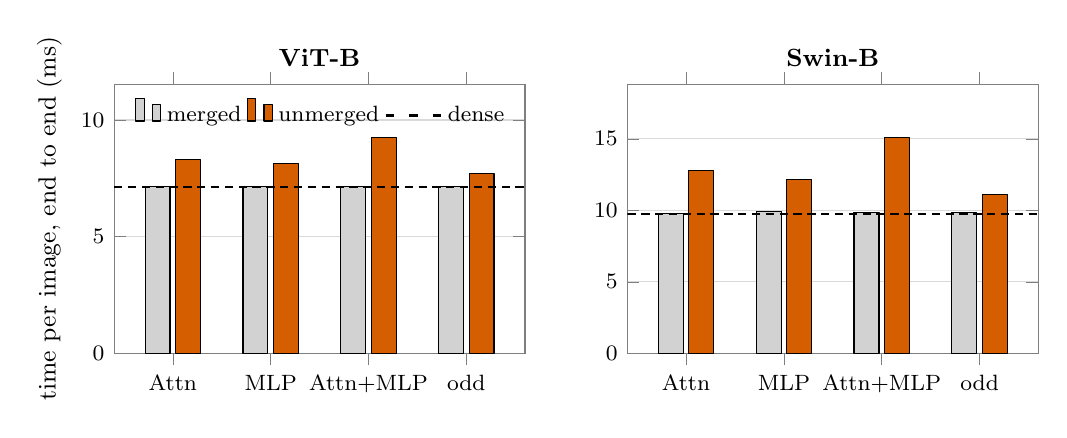
\begin{tikzpicture}
\begin{groupplot}[group style={group size=2 by 1, horizontal sep=\figSep, vertical sep=1.3cm}, width=\figW, height=\figH, repaxis, ybar, /pgf/bar width=9pt, ymin=0, xmin=0.4, xmax=4.6, xtick={1,2,3,4}, xticklabels={Attn,MLP,Attn+MLP,odd}, ymajorgrids, legend style={font=\footnotesize, draw=none, fill=none}, legend pos=north west, legend columns=-1, enlarge y limits={upper, value=0.25}]
\nextgroupplot[title={ViT-B}, ylabel={time per image, end to end (ms)}]
\addplot[fill=cGrey!35, draw=black] coordinates {(1,7.14) (2,7.14) (3,7.15) (4,7.13)};
\addlegendentry{merged}
\addplot[fill=cAccent, draw=black] coordinates {(1,8.29) (2,8.13) (3,9.23) (4,7.71)};
\addlegendentry{unmerged}
\draw[black, densely dashed, thick] (axis cs:0.4,7.12) -- (axis cs:4.6,7.12);
\addlegendimage{black, densely dashed, thick, line legend}
\addlegendentry{dense}
\nextgroupplot[title={Swin-B}]
\addplot[fill=cGrey!35, draw=black] coordinates {(1,9.80) (2,9.92) (3,9.83) (4,9.83)};
\addplot[fill=cAccent, draw=black] coordinates {(1,12.79) (2,12.14) (3,15.06) (4,11.12)};
\draw[black, densely dashed, thick] (axis cs:0.4,9.74) -- (axis cs:4.6,9.74);
\end{groupplot}
\end{tikzpicture}
\par}
\vspace{-1mm}
\begin{columns}[T]
\begin{column}{0.48\textwidth}
\footnotesize
\begin{itemize}
  \item $+$8 to $+$30\% (ViT-B), $+$14 to $+$55\% (Swin-B)
  \item \textbf{end to end}: preparing the image, copying it to the GPU, the forward pass, and copying the predicted class back
\end{itemize}
\end{column}
\begin{column}{0.48\textwidth}
\footnotesize
\begin{itemize}
  \item why: next slide
  \item in batches of 8 or more: 2--17\% (each launch serves the whole batch)
\end{itemize}
\end{column}
\end{columns}
\src{One test image end to end on the GPU, median over 9,950 images, 3 processes. Not an edge device.}
\end{frame}

% 14 -------------------------------------------------------------------------------------------------------------
\subsection{14. Why unmerged adapters are slow: many small GPU launches}
\begin{frame}{Why unmerged adapters are slow: many small GPU launches}
\vspace{-1mm}
{\renewcommand{\figH}{4.0cm}\centering% generated by scripts/make_figures.py; do not edit
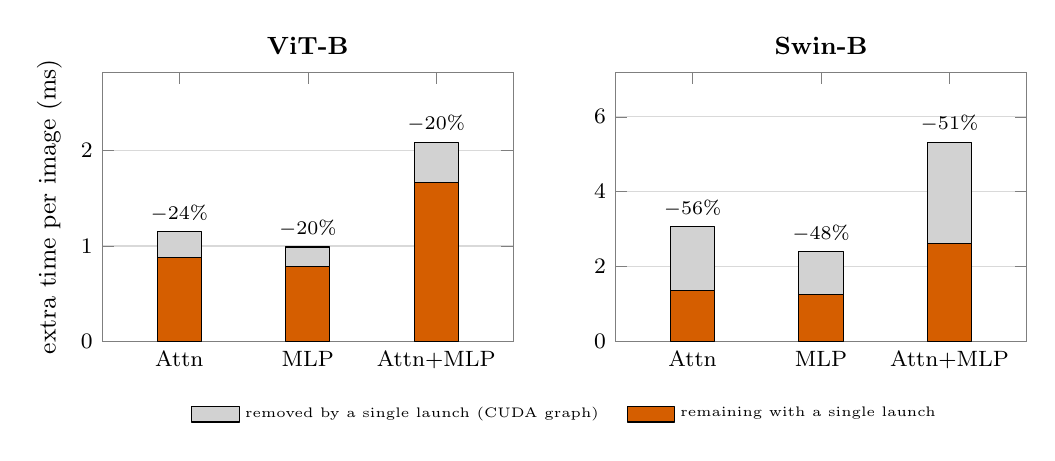
\begin{tikzpicture}
\begin{groupplot}[group style={group size=2 by 1, horizontal sep=\figSep, vertical sep=1.3cm}, width=\figW, height=\figH, repaxis, ybar stacked, /pgf/bar width=16pt, ymin=0, xmin=0.4, xmax=3.6, xtick={1,2,3}, xticklabels={Attn,MLP,Attn+MLP}, ymajorgrids, enlarge y limits={upper, value=0.35}, legend style={font=\figLegendFont, draw=none, fill=none, at={(-0.12,-0.2)}, anchor=north, legend columns=-1, /tikz/every even column/.append style={column sep=8pt}}]
\nextgroupplot[title={ViT-B}, ylabel={extra time per image (ms)}]
\addplot[fill=cAccent, draw=black, forget plot] coordinates {(1,0.877) (2,0.788) (3,1.665)};
\addplot[fill=cGrey!35, draw=black, forget plot] coordinates {(1,0.272) (2,0.202) (3,0.424)};
\node[font=\scriptsize, anchor=south] at (axis cs:1,1.149) {$-$24\%};
\node[font=\scriptsize, anchor=south] at (axis cs:2,0.990) {$-$20\%};
\node[font=\scriptsize, anchor=south] at (axis cs:3,2.089) {$-$20\%};
\nextgroupplot[title={Swin-B}]
\addplot[fill=cAccent, draw=black, forget plot] coordinates {(1,1.354) (2,1.244) (3,2.614)};
\addplot[fill=cGrey!35, draw=black, forget plot] coordinates {(1,1.704) (2,1.155) (3,2.711)};
\node[font=\scriptsize, anchor=south] at (axis cs:1,3.058) {$-$56\%};
\node[font=\scriptsize, anchor=south] at (axis cs:2,2.399) {$-$48\%};
\node[font=\scriptsize, anchor=south] at (axis cs:3,5.325) {$-$51\%};
\addlegendimage{area legend, fill=cGrey!35, draw=black}
\addlegendentry{removed by a single launch (CUDA graph)}
\addlegendimage{area legend, fill=cAccent, draw=black}
\addlegendentry{remaining with a single launch}
\end{groupplot}
\end{tikzpicture}
\par}
\vspace{-1mm}
\begin{columns}[T]
\begin{column}{0.48\textwidth}
\footnotesize
\begin{itemize}
  \item the CPU starts every GPU operation separately; each \textbf{launch} has a fixed cost of a few $\mu$s
  \item unmerged adapters add many small operations: two small matrix products, a scaling and an addition per adapted weight
\end{itemize}
\end{column}
\begin{column}{0.48\textwidth}
\footnotesize
\begin{itemize}
  \item a \textbf{CUDA graph} replays the whole forward pass as one launch: the same computation, without the per-launch cost
  \item launch overhead is \textbf{48--56\%} of the extra time on Swin-B, \textbf{20--24\%} on ViT-B; the rest was not broken down
\end{itemize}
\end{column}
\end{columns}
\src{Forward pass of one test image, extra time over the dense model, median over 9,950 images, 3 processes. The graph is a diagnostic only.}
\end{frame}

% 15 --------------------------------------------------------------------------------------------------------------
\subsection{15. Closing study: training memory can be predicted}
\begin{frame}{Closing study: training memory can be predicted}
\begin{columns}[T]
\begin{column}{0.50\textwidth}
\renewcommand{\figWone}{6.2cm}
\centering% generated by scripts/make_figures.py; do not edit
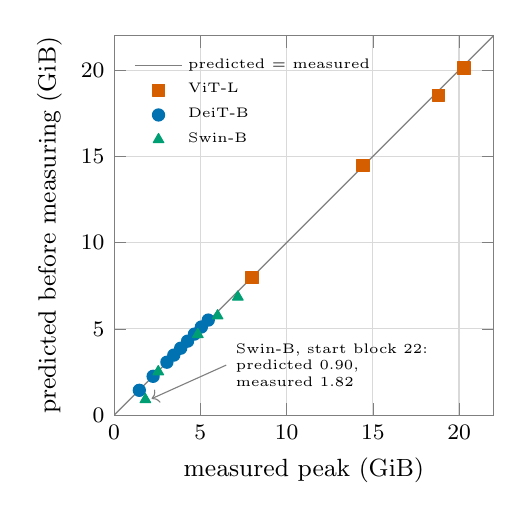
\begin{tikzpicture}
\begin{axis}[width=\figWone, height=\figWone, repaxis, xmin=0, xmax=22, ymin=0, ymax=22, xlabel={measured peak (GiB)}, ylabel={predicted before measuring (GiB)}, grid=major, legend style={font=\figLegendFont, draw=none, fill=none, legend cell align=left}, legend pos=north west]
\addplot[cGrey, domain=0:22, samples=2] {x};
\addlegendentry{predicted = measured}
\addplot[cAccent, only marks, mark=square*, mark size=2.2pt] coordinates {(20.287,20.12) (14.436,14.48) (8.003,7.96) (18.830,18.55)};
\addlegendentry{ViT-L}
\addplot[cAttn, only marks, mark=*, mark size=2.2pt] coordinates {(5.459,5.51) (5.059,5.11) (1.462,1.44) (4.660,4.70) (4.260,4.29) (3.860,3.88) (3.461,3.48) (3.061,3.07) (2.262,2.25)};
\addlegendentry{DeiT-B}
\addplot[cBoth, only marks, mark=triangle*, mark size=2.2pt] coordinates {(2.560,2.52) (7.175,6.85) (1.815,0.90) (6.000,5.76) (4.854,4.68)};
\addlegendentry{Swin-B}
\node[font=\figLegendFont, anchor=west, align=left] (miss) at (axis cs:6.5,2.90) {Swin-B, start block 22:\\predicted 0.90,\\measured 1.82};
\draw[->, cGrey] (miss.west) -- (axis cs:2.17,0.95);
\end{axis}
\end{tikzpicture}

\end{column}
\begin{column}{0.46\textwidth}
\footnotesize
\textbf{Question}: given a limit on training memory, where can the adapters start?
\begin{itemize}
  \item a formula with three constants and a small term per image, fitted on ViT-B, from the shape of the model
  \item predictions \textbf{written down before measuring}
  \item ViT-L (a new shape): within \textbf{1.5\%}; Swin-B, start blocks 2--16: within \textbf{4.6\%}
  \item one miss: Swin-B with adapters on the last two blocks only (temporary memory of the forward pass sets the peak)
\end{itemize}
\medskip
Which placement is the most accurate under a budget is still open (future work).
\end{column}
\end{columns}
\end{frame}

% 16 --------------------------------------------------------------------------------------------------------------
\subsection{16. Conclusions and limitations}
\begin{frame}{Conclusions and limitations}
\begin{columns}[T]
\begin{column}{0.56\textwidth}
\small
\begin{enumerate}
  \item \textbf{Accuracy}: with both methods tuned, LoRA is ahead on Swin-B; on ViT-B it is level or slightly behind, with no evidence that LoRA is better.
  \item \textbf{Training}: attention LoRA needs a third less memory at batch 64, about 70\% less at batch 1, and has about a quarter shorter epochs.
  \item \textbf{Placement}: the first adapted block sets the memory; adapting only the later half costs 1.2--1.6 pp.
  \item \textbf{Deployment}: merge for a single task; keep adapters separate only to share a base model.
\end{enumerate}
\end{column}
\begin{column}{0.4\textwidth}
\small
\textbf{Limitations}
\begin{itemize}
  \item one dataset (CIFAR-100, close to saturated)
  \item 32-bit floats, a shared server GPU; no edge device
  \item power could not be measured per job
  \item 3 seeds for the learning-rate check and DeiT-B
  \item causes not tested
\end{itemize}
\end{column}
\end{columns}
\vfill{\centering\scriptsize Code and all results: \url{https://github.com/Photon-139/rnd-project}\par}
\end{frame}

% ==================================================================================================================
\appendix
\section{Backup slides}
\begin{frame}[plain]
\centering\Large\bfseries\color{cInk} Backup slides
\end{frame}

\subsection{18. Learning-rate check, all numbers (3 seeds)}
\begin{frame}{Backup: learning-rate check, all numbers (3 seeds)}
\centering\scriptsize
\begin{tabular}{llccc}
\toprule
method & learning rate & validation loss & test acc.\ (\%) & stopping epoch \\
\midrule
\rawinput{../final_report/data/tab_lr.tex}
\bottomrule
\end{tabular}
\src{$^*$ lowest validation loss of the method on that model. ViT-B full FT at $10^{-4}$: an earlier set of runs.}
\end{frame}

\subsection{19. How far to trust the ViT-B difference}
\begin{frame}{Backup: how far to trust the ViT-B difference}
\small
\begin{columns}[T]
\begin{column}{0.56\textwidth}
\textbf{Attention LoRA $-$ full fine-tuning on ViT-B} (pp, paired)\par\smallskip
\begin{tabular}{@{}lc@{}}
\toprule
at $10^{-4}$, 5 seeds & $-$0.21 $\pm$ 0.13 \\
at $3{\times}10^{-4}$ (same val.\ loss), 3 seeds & $+$0.08 $\pm$ 0.27 \\
at $10^{-4}$, repeated set of runs, 3 seeds & $-$0.04 $\pm$ 0.29 \\
\bottomrule
\end{tabular}
\par\smallskip
\begin{itemize}
  \item the repeated set is 0.19 pp above the main runs on the same seeds: run-to-run variation is as large as the difference
\end{itemize}
\end{column}
\begin{column}{0.41\textwidth}
\textbf{Validation loss}, LoRA $-$ full FT\par\smallskip
\begin{tabular}{@{}lcc@{}}
\toprule
 & ViT-B & Swin-B \\
\midrule
Attn & $-$0.031 & $-$0.018 \\
MLP & $-$0.026 & $-$0.018 \\
Attn+MLP & $-$0.028 & $-$0.019 \\
\bottomrule
\end{tabular}
\par\smallskip
{\footnotesize Lower in all 30 seed pairs. On ViT-B this does not turn into higher test accuracy.}
\end{column}
\end{columns}
\take{Against an untuned full fine-tuning ($10^{-5}$), LoRA would have looked 0.4--0.7 pp better on ViT-B.}
\end{frame}

\subsection{20. Rank 16 gives no gain on ViT-B}
\begin{frame}{Backup: rank 16 gives no gain on ViT-B}
\small\centering
\begin{tabular}{lccccc}
\toprule
 & \multicolumn{2}{c}{test acc.\ (\%)} & rank 16 $-$ rank 8 & \multicolumn{2}{c}{peak memory (GiB)} \\
target & rank 8 & rank 16 & (pp, paired) & rank 8 & rank 16 \\
\midrule
Attn & 91.21 & 91.06 & $-$0.15 $\pm$ 0.12 & 5.459 & 5.478 \\
MLP & 91.31 & 91.30 & $-$0.02 $\pm$ 0.13 & 7.011 & 7.028 \\
Attn+MLP & 91.44 & 91.50 & $+$0.05 $\pm$ 0.12 & 7.644 & 7.679 \\
\bottomrule
\end{tabular}
\par\medskip
\begin{itemize}
  \item 5 seeds, library implementation. Attention: lower with rank 16 in the library runs (5 of 5 seeds), but $+$0.02 $\pm$ 0.04 pp in our own implementation
  \item memory rises by less than 0.04 GiB
  \item ViT-B only; rank 16 was not run on Swin-B
\end{itemize}
\end{frame}

\subsection{21. Which target is most accurate? Only at rate 1e-4}
\begin{frame}{Backup: which target is most accurate? Only ``at rate $10^{-4}$''}
\small
\begin{itemize}
  \item \textbf{Swin-B}: no clear difference between attention, MLP and both ($-$0.05 to $+$0.01 pp)
  \item \textbf{ViT-B} at $10^{-4}$: MLP $+$0.25 $\pm$ 0.16 pp and Attn+MLP $+$0.33 $\pm$ 0.16 pp above attention, 5 of 5 seeds
  \item But at rate $3\times10^{-4}$ (same validation loss) attention is level with them: $+$0.13 $\pm$ 0.24 pp against MLP, $-$0.07 $\pm$ 0.24 pp against Attn+MLP (3 seeds)
\end{itemize}
\take{We do not claim that the MLP is the better target. The cost difference is the robust result.}
\end{frame}

\subsection{22. Placement accuracies (5 seeds, paired against all blocks)}
\begin{frame}{Backup: placement accuracies (5 seeds, paired against all blocks)}
\small\centering
\begin{tabular}{lcccc}
\toprule
 & \multicolumn{2}{c}{ViT-B} & \multicolumn{2}{c}{Swin-B} \\
placement & test acc.\ (\%) & vs all (pp) & test acc.\ (\%) & vs all (pp) \\
\midrule
all blocks & 91.10 $\pm$ 0.08 & -- & 91.74 $\pm$ 0.31 & -- \\
first half & 91.31 $\pm$ 0.11 & $+$0.21 $\pm$ 0.06 & 91.36 $\pm$ 0.20 & $-$0.38 $\pm$ 0.20 \\
even & 91.05 $\pm$ 0.08 & $-$0.06 $\pm$ 0.09 & 91.72 $\pm$ 0.19 & $-$0.03 $\pm$ 0.42 \\
odd & 90.89 $\pm$ 0.22 & $-$0.22 $\pm$ 0.23 & 91.82 $\pm$ 0.29 & $+$0.08 $\pm$ 0.27 \\
second half & 89.54 $\pm$ 0.13 & $-$1.56 $\pm$ 0.15 & 90.57 $\pm$ 0.19 & $-$1.18 $\pm$ 0.19 \\
full FT & 91.31 $\pm$ 0.15 & $+$0.21 $\pm$ 0.13 & 91.26 $\pm$ 0.23 & $-$0.48 $\pm$ 0.28 \\
\bottomrule
\end{tabular}
\par\medskip
Even blocks: within the spread over seeds of all blocks on both models (not equivalence; Swin-B has one seed at $+$0.72 pp).
\end{frame}

\subsection{23. Odd blocks, a cheap saving}
\begin{frame}{Backup: odd blocks, a cheap saving}
\small
\centering
\setlength{\tabcolsep}{4pt}
\begin{tabular}{@{}lccc@{}}
\toprule
odd blocks vs all blocks & accuracy (pp, paired) & peak memory (GiB) & train epoch \\
\midrule
ViT-B & $-$0.22 $\pm$ 0.23 \ (4 of 5 seeds lower) & 4.87 vs 5.46 \ ($-$11\%) & $-$8\% \\
Swin-B & $+$0.08 $\pm$ 0.27 \ (2 of 5 seeds lower) & 8.18 vs 9.55 \ ($-$14\%) & $-$8\% \\
\bottomrule
\end{tabular}
\par\bigskip
\begin{columns}[T]
\raggedright
\begin{column}{0.47\textwidth}
\begin{itemize}
  \item Accuracy within the spread over seeds of all blocks, on both models
  \item \alert{Not the same as no loss}: on ViT-B the mean is negative and the validation loss is worse in 5 of 5 seeds
\end{itemize}
\end{column}
\begin{column}{0.47\textwidth}
\begin{itemize}
  \item 60--70\% of the saving comes from not reaching block 0
  \item The second half saves far more (44\% and 61\%) but loses 1.2--1.6 pp
\end{itemize}
\end{column}
\end{columns}
\end{frame}

\subsection{24. Throughput, CPU latency and task switching}
\begin{frame}{Backup: throughput, CPU latency and task switching}
\small
\begin{columns}[T]
\begin{column}{0.5\textwidth}
\textbf{Unmerged penalty in throughput} (images per second) against batch size; slide 13 is a different measure, time per image end to end\par\smallskip
\begin{tabular}{@{}lcc@{}}
\toprule
 & batch 1 & batch 8 or more \\
\midrule
ViT-B & 8--25\% & 2--13\% \\
Swin-B & 13--37\% & 2--17\% \\
\bottomrule
\end{tabular}
\par\medskip
\textbf{CPU} (4 threads, one image): unmerged $+$1 to $+$15\% (ViT-B), $+$4 to $+$24\% (Swin-B). One process, 190 images; the low end is within noise.
\end{column}
\begin{column}{0.46\textwidth}
\textbf{Switching tasks}
\begin{itemize}
  \item load and apply an adapter: 2.6--7.9 ms (ViT-B), 5.4--16.3 ms (Swin-B)
  \item load a full model: 91--100 ms, 108--133 ms
  \item files already in memory: lower bounds
\end{itemize}
\medskip
\textbf{CUDA graph} removes 48--62\% of the unmerged penalty on Swin-B and 20--27\% on ViT-B.
\end{column}
\end{columns}
\end{frame}

\subsection{25. Our own implementation agrees with the library}
\begin{frame}{Backup: our own implementation agrees with the library}
\small
Every ViT-B LoRA configuration was trained twice per seed: HuggingFace + PEFT, and our own ViT and LoRA code, from identical initial weights.
\begin{itemize}
  \item mean accuracy differs by at most \textbf{0.08 pp}; single seeds by at most 0.26 pp
  \item peak memory differs by at most \textbf{0.003 GiB}
  \item same stopping epoch in 32 of 35 seed pairs; identical trainable-parameter counts
\end{itemize}
\medskip
\textbf{Run-to-run variation}: the same ViT-B configuration and seeds trained again differ by 0.04--0.15 pp per seed (one run 0.36 pp), and by 0.1--0.2 pp in the mean. Differences of about 0.2 pp cannot be shown or excluded with 5 seeds.
\end{frame}

\subsection{26. The accuracy rule for a later start, and why it failed}
\begin{frame}{Backup: the accuracy rule for a later start, and why it failed}
\small
\textbf{Rule}, written down before the runs: $\Delta\text{acc}(k) \approx -\beta\,k/L$ against adapters on all blocks; $\beta$ from the second-half results ($k/L=0.5$): 3.1 (ViT-B), 2.4 (Swin-B), average 2.7 pp. Ranges $\pm$0.6 pp by judgement.
\par\medskip\centering\footnotesize
\begin{tabular}{lccccc}
\toprule
attention LoRA & all blocks & blocks $k$ on & predicted & measured & within? \\
 & (\%) & (\%) & (pp) & (pp, 3 seeds) & \\
\midrule
DeiT-B, $k=3$ & 86.56 & 86.71 & $-$0.7 ($-$1.4 to $-$0.2) & $+$0.15 $\pm$ 0.04 & \alert{no} \\
DeiT-B, $k=6$ & 86.56 & 86.24 & $-$1.4 ($-$2.5 to $-$0.7) & $-$0.32 $\pm$ 0.35 & \alert{no} \\
ViT-B, $k=3$  & 91.28 & 90.97 & $-$0.8 ($-$1.4 to $-$0.2) & $-$0.31 $\pm$ 0.27 & at the edge \\
\bottomrule
\end{tabular}
\par\medskip\raggedright\small
\begin{itemize}
  \item a later start cost \textbf{less} than predicted; start at block 3: 22\% less memory, 14\% shorter epochs
  \item the memory and time predictions for the same runs all held
\end{itemize}
\end{frame}

\subsection{27. The memory formula and its one miss}
\begin{frame}{Backup: the memory formula and its one miss}
\small
\[
\text{peak} = \text{resident} + B\cdot\Big(c_\text{reach}\!\sum_{b\ge k}\! s_b + c_\text{attn}\!\!\sum_{\text{attn}}\! s_b + c_\text{mlp}\!\!\sum_{\text{MLP}}\! s_b + h\Big),\qquad s_b = \text{tokens}\times\text{width}\times 4\ \text{bytes}
\]
\begin{itemize}
  \item fitted on 7 ViT-B configurations: $c_\text{reach}=9.95$, $c_\text{attn}=1.34$, $c_\text{mlp}=4.86$; $h$ = memory per image of the layers outside the blocks, fitted at 4 MiB
  \item memory is linear in the batch size (within 0.005 GiB on ViT-B, 0.04 GiB on Swin-B) and identical across seeds
  \item ViT-L: mean error 0.8\%, largest 1.5\%; three predicted out-of-memory cases all happened
  \item DeiT-B: within 1.7\% (same shape as ViT-B, a consistency check)
  \item \alert{Miss}: Swin-B with adapters on the last two blocks: predicted 0.90, measured 1.82 GiB. The peak there is temporary memory of the forward pass through the large early stages; the formula needs a lower bound for it
\end{itemize}
\end{frame}

\subsection{28. Other ways to meet a budget}
\begin{frame}{Backup: other ways to meet a budget}
\small
\textbf{Gradient accumulation}
\begin{itemize}
  \item process the batch in pieces and add the gradients: memory follows the piece size
  \item same update for ViT-B / DeiT-B (per-token normalisation, no dropout): an argument, not run
  \item then placement mainly buys \textbf{time}: epochs 14\% (block 3) to 28\% (block 6) shorter
  \item step time of accumulation and gradient checkpointing: not measured
\end{itemize}
\end{frame}

\subsection{29. Why power was not measured}
\begin{frame}{Backup: why power was not measured}
\small
\begin{itemize}
  \item Our jobs run on one partition (MIG slice) of a shared NVIDIA B200
  \item The GPU reports power only for the \textbf{whole card}, including other users' jobs; power per partition is ``not supported''; the cluster records no energy per job
  \item Test: 30 s idle / 30 s steady load, alternating. The card drew 280--503 W while our partition was idle; our load added 6--78 W, not repeatably
\end{itemize}
\take{The energy of one job cannot be separated from the card's. It needs an exclusive card or an edge device.}
\end{frame}

\end{document}
